\chapter{Background and Theoretical Foundations}
\label{Background}

\section{Introduction to Fourier Transform}
In mathematics, the Fourier transform (FT) is an integral transform that acts on a function to reveal its frequency components. It takes an input function and generates a new, complex-valued function that details the intensity of different frequencies present in the original. The term ``Fourier transform'' applies to both the mathematical process itself and the resulting function. To distinguish between the two, the output is often referred to as the ``frequency domain'' representation~\cite{oppenheim2010}.. 

\begin{figure}[H]
    \centering
    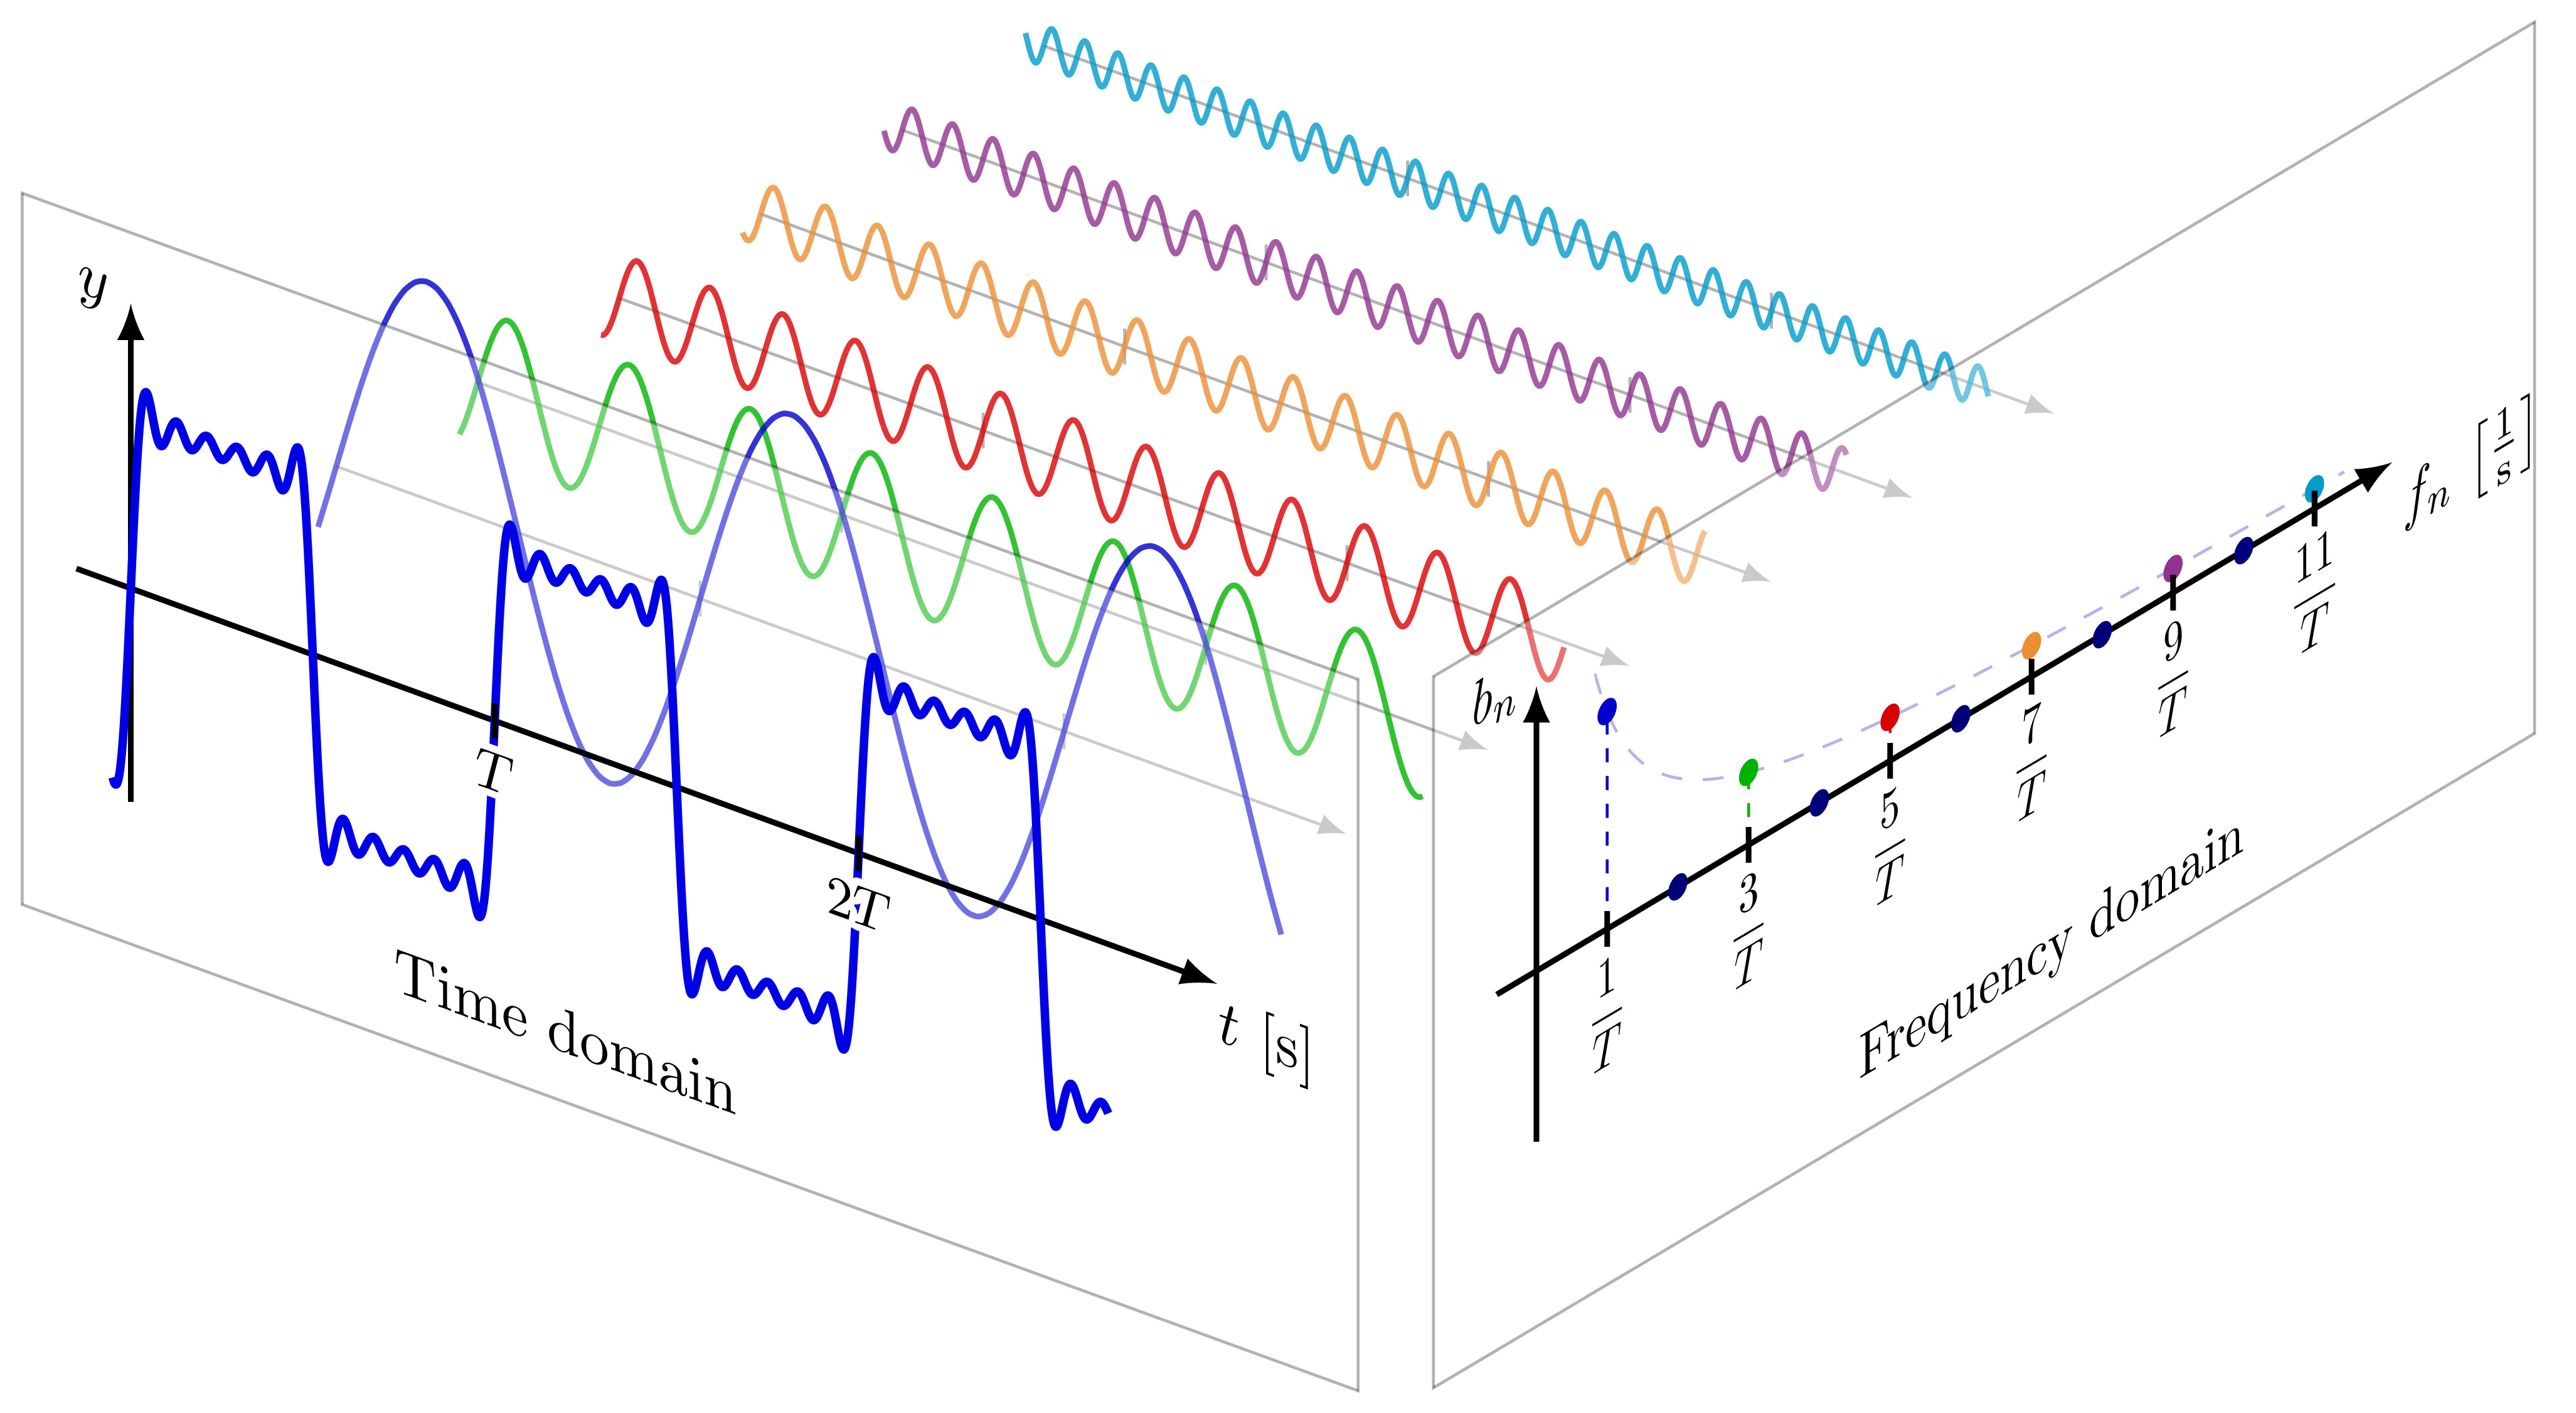
\includegraphics[width=0.6\linewidth]{Images/fourier_transform.jpeg}
    \caption{Representation of a time-domain signal decomposed into multiple signals of different frequencies.}
    \label{fig:time_domain_decomp}
\end{figure}

The Fourier transform, $\hat{f}(\omega)$, of a function $f(t)$ is defined mathematically as:

\begin{equation}
    \hat{f}(\omega) = \int_{-\infty}^{\infty} f(t) e^{-i\omega t} \, dt
\end{equation}

\section{Fast Fourier Transform in General}
The Fast Fourier Transform (FFT) is an efficient algorithm used to compute the Discrete Fourier Transform (DFT) of a sequence, which transforms a signal from the time domain into the frequency domain. This means it breaks down a complex signal into its constituent sinusoidal components, frequencies and their amplitudes, making it easier to analyze patterns such as pitch in audio, frequencies in communications, or periodicities in data. The FFT drastically reduces the computational complexity of DFT from $O(N^2)$ to $O(N\log(N))$ by cleverly reusing calculations through a divide-and-conquer approach. This algorithm is ideal for real-life applications like audio processing, image analysis, wireless communication, and other biomedical and industrial applications.

The most common FFT algorithm is the \textbf{Cooley-Tukey} algorithm~\cite{cooley1965}, which is widely used due to its simplicity and efficiency. It works best when the input size $N$ is a power of 2. The most common versions of the algorithm are:

\begin{itemize}
    \item \textbf{Radix-2}: The most basic and common version. Splits the DFT into two halves (even and odd indices) at each stage. Requires $N$ to be a power of 2.
    \item \textbf{Radix-4}: More efficient than Radix-2 when $N$ is a power of 4. Reduces the number of multiplications compared to Radix-2 by grouping four elements at a time.
    \item \textbf{Split-Radix}: This combines both Radix-2 and Radix-4 versions in order to improve computational efficiency.
\end{itemize}

\begin{figure}[H]
    \centering
    
    % Top row: Radix-2 and Radix-4
    \begin{subfigure}[t]{0.48\linewidth}
        \centering
        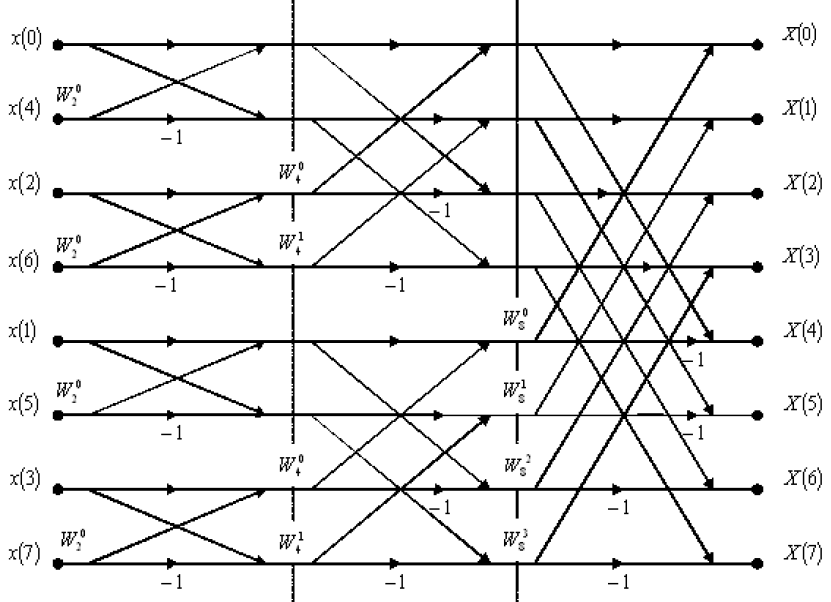
\includegraphics[width=\linewidth]{Images/r2.png}
        \caption{Radix-2 Dataflow}
        \label{fig:radix2_dataflow}
    \end{subfigure}
    \hfill
    \begin{subfigure}[t]{0.48\linewidth}
        \centering
        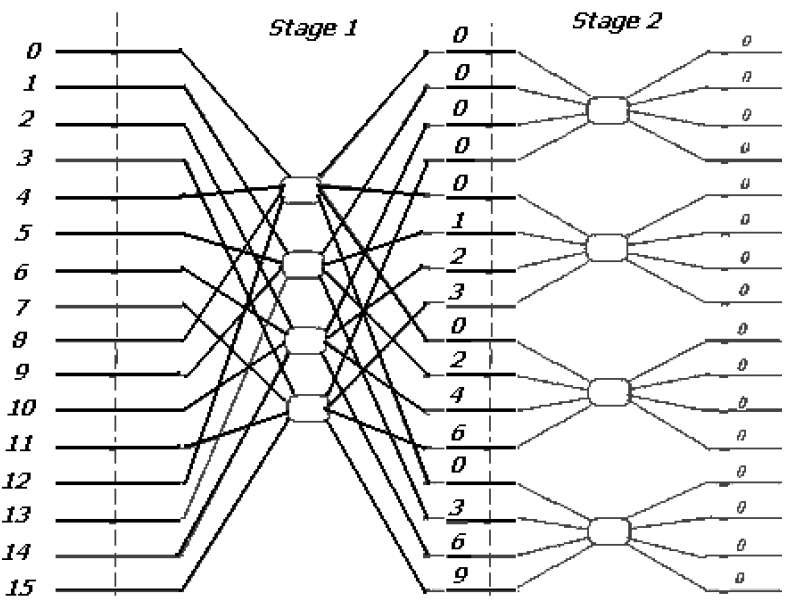
\includegraphics[width=\linewidth]{Images/r4.png}
        \caption{Radix-4 Dataflow}
        \label{fig:radix4_dataflow}
    \end{subfigure}
    
    \vspace{1em} % Adds a little space between the rows
    
    % Bottom row: Third image
    \begin{subfigure}[t]{\linewidth}
        \centering
        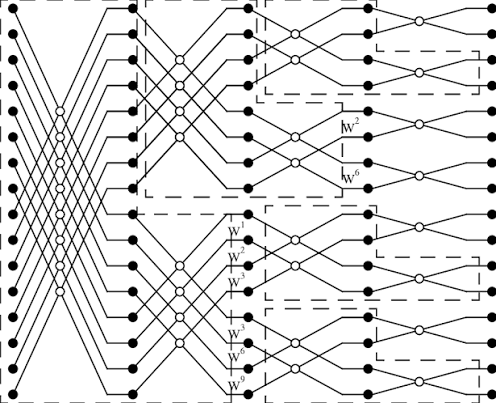
\includegraphics[width=0.6\linewidth]{Images/r_s.png}
        \caption{Split-Radix Dataflow}
        \label{fig:r_s_dataflow}
    \end{subfigure}
    
    % Main caption and label for the entire figure
    \caption{Comparison of Radix-2, Radix-4 and Split-Radix dataflow structures.}
    \label{fig:FFT_dataflows}
\end{figure}

\section{FFT Decomposition}
\subsection{Radix-2}

Given a sequence $x[n]$ of length $N$, the Discrete Fourier Transform (DFT) is defined as~\cite{oppenheim2010}:
\begin{equation}
    X[k] = \sum_{n=0}^{N-1} x[n] \cdot W_N^{kn}, \quad \text{where } W_N = e^{-j\frac{2\pi}{N}}
\end{equation}
Here, $W_N$ represents the \textbf{twiddle factor}. The primary advantage of the FFT algorithm is its ability to reorganize this summation, thereby drastically reducing the overall computational complexity.

By separating the input data $x[n]$ into even-indexed ($e[n] = x[2n]$) and odd-indexed ($o[n] = x[2n+1]$) elements, the DFT can be expressed as:
\begin{equation}
    X[k] = \sum_{n=0}^{N/2 - 1} x[2n] \cdot W_N^{k \cdot 2n} + \sum_{n=0}^{N/2 - 1} x[2n+1] \cdot W_N^{k \cdot (2n+1)}
\end{equation}
Applying the substitution $W_N^{2kn} = W_{N/2}^{kn}$, we can factor the equation into two smaller transforms:
\begin{equation}
    X[k] = \underbrace{\sum_{n=0}^{N/2 - 1} e[n] \cdot W_{N/2}^{kn}}_{\text{Even terms } (E[k])} + W_N^k \cdot \underbrace{\sum_{n=0}^{N/2 - 1} o[n] \cdot W_{N/2}^{kn}}_{\text{Odd terms } (O[k])}
\end{equation}
Let $E[k]$ and $O[k]$ represent the DFTs of the even and odd sequences, respectively. This reduces the main equation to:
\begin{equation}
    X[k] = E[k] + W_N^k \cdot O[k]
\end{equation}
Exploiting the $N$-periodicity of the DFT, the complete range for $k = 0, 1, \dots, N-1$ is evaluated using the standard \textbf{butterfly operation}:
\begin{align}
    X[k] &= E[k] + W_N^k \cdot O[k] \\
    X\left[k + \frac{N}{2}\right] &= E[k] - W_N^k \cdot O[k]
\end{align}
for $k = 0, 1, \dots, N/2 - 1$. For an input sequence where $N = 2^m$, this algorithm completes the transform in $m = \log_2(N)$ stages by recursively applying these butterfly operations.

\begin{figure}[H]
    \centering
    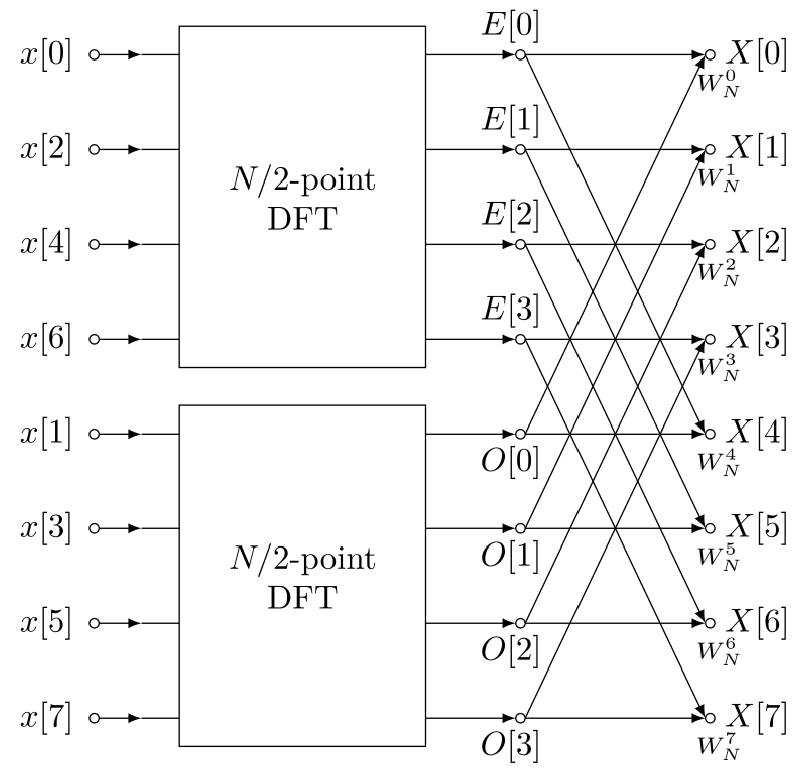
\includegraphics[width=0.4\textwidth]{Images/fft_rec.png} 
    \caption{Recursive logic of the Radix-2 FFT, demonstrating the combination of even and odd sequences from previous stages.}
    \label{fig:radix2_rec}
\end{figure}

\subsection{Radix-4}

The Radix-4 FFT builds upon the fundamental principles of Radix-2 by partitioning the DFT into \textbf{four smaller DFTs}. This requires the input sequence length $N$ to be a power of 4 (i.e., $N=4^m$).

The input sequence $x[n]$ is divided into four interleaved subsequences:
\begin{align}
    x_0[n] &= x[4n], & x_1[n] &= x[4n+1], \nonumber \\
    x_2[n] &= x[4n+2], & x_3[n] &= x[4n+3]
\end{align}
Expanding the DFT with these subsequences yields:
\begin{equation}
    X[k] = \sum_{n=0}^{N/4-1} \left[ 
    x[4n] + x[4n+1] W_N^k + x[4n+2] W_N^{2k} + x[4n+3] W_N^{3k}
    \right] W_{N/4}^{kn}
\end{equation}
This equation effectively acts as a linear combination of four $N/4$-point DFTs, denoted as $X_0, X_1, X_2, \text{ and } X_3$:
\begin{equation}
    X[k] = X_0[k] + W_N^k X_1[k] + W_N^{2k} X_2[k] + W_N^{3k} X_3[k]
\end{equation}
To streamline the 4-point butterfly calculation, we define four intermediate variables:
\begin{equation}
    A = X_0[k], \quad B = W_N^k X_1[k], \quad C = W_N^{2k} X_2[k], \quad D = W_N^{3k} X_3[k]
\end{equation}
The resulting butterfly outputs are computed as follows:
\begin{align}
    X[k] &= A + B + C + D \\
    X\left[k + \frac{N}{4}\right] &= A - jB - C + jD \\
    X\left[k + \frac{N}{2}\right] &= A - B + C - D \\
    X\left[k + \frac{3N}{4}\right] &= A + jB - C - jD
\end{align}
By leveraging additional symmetries, the Radix-4 algorithm lowers the total number of stages to $\log_4(N)$. This significantly reduces the multiplication count compared to Radix-2, making it highly efficient for hardware implementations when applicable.

\subsection{Split-Radix}

The \textbf{Split-Radix FFT (SRFFT)} elegantly combines the structures of Radix-2 and Radix-4 to achieve superior computational efficiency. It relies on the mathematical observation that the even-indexed terms of the DFT are best computed using a Radix-2 approach, while the odd-indexed terms are more efficiently handled using a Radix-4 approach. This method yields the lowest number of arithmetic operations for power-of-two FFTs.

The standard DFT is decomposed by applying a Radix-2 split to the even indices, and a Radix-4 split to the odd indices:
\begin{equation}
    X[k] = \sum_{n=0}^{N/2-1} x[2n] W_{N/2}^{kn} + \sum_{n=0}^{N/4-1} x[4n+1] W_N^{k(4n+1)} + \sum_{n=0}^{N/4-1} x[4n+3] W_N^{k(4n+3)}
\end{equation}
By factoring out the twiddle factors for the odd terms, the equation simplifies to:
\begin{equation}
    X[k] = \sum_{n=0}^{N/2-1} x[2n] W_{N/2}^{kn} + W_N^k \sum_{n=0}^{N/4-1} x[4n+1] W_{N/4}^{kn} + W_N^{3k} \sum_{n=0}^{N/4-1} x[4n+3] W_{N/4}^{kn}
\end{equation}
Let $E[k]$ be the $N/2$-point DFT of the even elements, and let $O_1[k]$ and $O_3[k]$ represent the $N/4$-point DFTs of the two interleaved odd sequences. The Split-Radix butterfly operation computes four outputs simultaneously using an L-shaped structure:
\begin{align}
    X[k] &= E[k] + \left( W_N^k O_1[k] + W_N^{3k} O_3[k] \right) \\
    X\left[k + \frac{N}{2}\right] &= E[k] - \left( W_N^k O_1[k] + W_N^{3k} O_3[k] \right) \\
    X\left[k + \frac{N}{4}\right] &= E\left[k + \frac{N}{4}\right] - j \left( W_N^k O_1[k] - W_N^{3k} O_3[k] \right) \\
    X\left[k + \frac{3N}{4}\right] &= E\left[k + \frac{N}{4}\right] + j \left( W_N^k O_1[k] - W_N^{3k} O_3[k] \right)
\end{align}
Because it selectively applies the most efficient decomposition step at each stage, the Split-Radix algorithm requires up to one third fewer multiplications than standard Radix-2~\cite{duhamel1984}, without placing the strict $N=4^m$ size restriction required by pure Radix-4.

\section{Unrolled and Single-Path Delay Feedback Approaches}
There are different approaches to designing the FFT algorithm in hardware. The most intuitive method is the unrolled architecture, which exploits inherent parallelism by unrolling the entire computation. Each butterfly operation is assigned a dedicated hardware unit, resulting in a fully unrolled design where all butterfly computations are executed concurrently. This method is very demanding in resources, especially for smaller FPGAs. Furthermore, it requires a very high data bandwidth, as a 256-point FFT would typically require access to 256 data points in the same clock cycle. For example, if each complex sample is 32 bits (16bits real and 16bits imaginary) long and the FFT operates at 100 MHz, the system requires a continuous bandwidth of 819.2 Gbps to run without stalling.

\begin{figure}[htbp]
    \centering
    \begin{subfigure}[t]{0.48\linewidth}
        \centering
        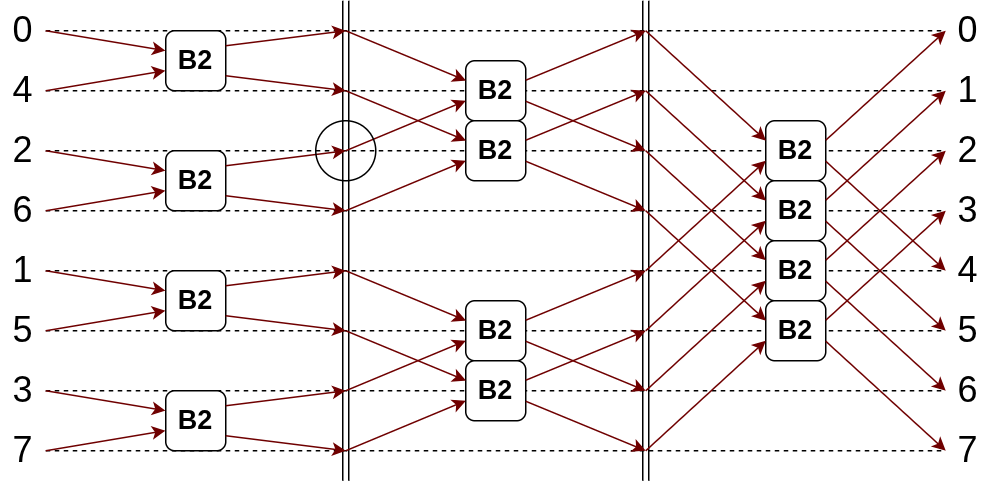
\includegraphics[width=\linewidth]{Images/r2_.png}
        \caption{Structure/dataflow of the Radix-2 unrolled algorithm (B2 = Butterfly 2).}
        \label{fig:radix2_unrolled}
    \end{subfigure}
    \hfill
    \begin{subfigure}[t]{0.48\linewidth}
        \centering
        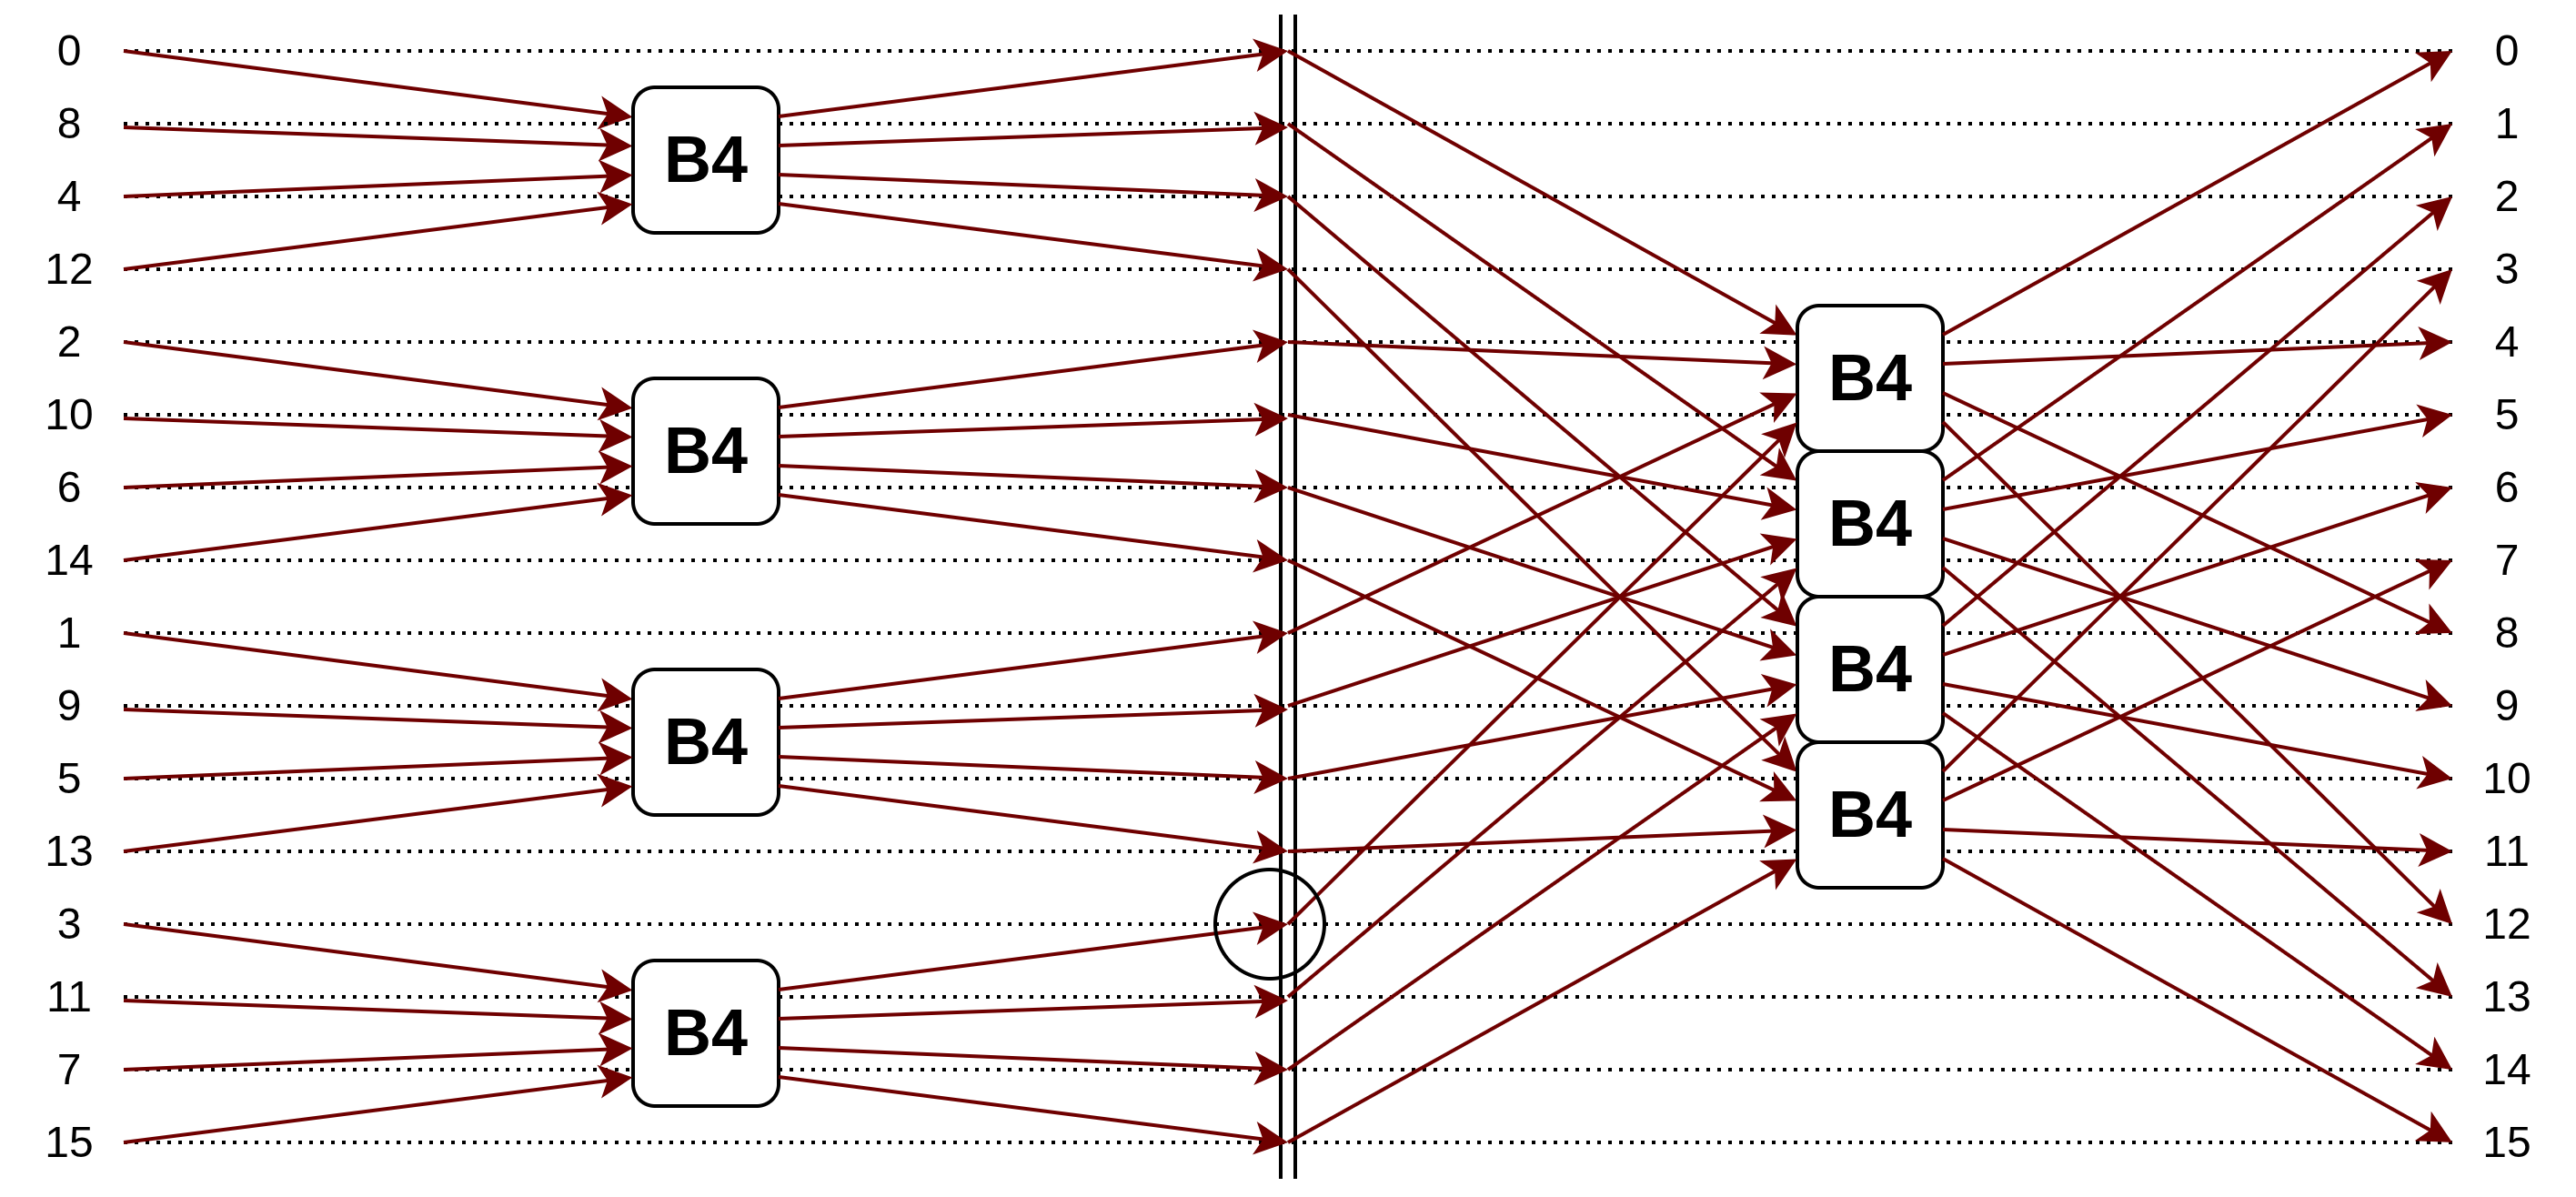
\includegraphics[width=\linewidth]{Images/r4.drawio_1.png}
        \caption{Structure/dataflow of the Radix-4 unrolled algorithm (B4 = Butterfly 4).}
        \label{fig:radix4_unrolled}
    \end{subfigure}
    \caption{Comparison of unrolled architectures.}
\end{figure}

A highly resource-efficient alternative allocates only a single butterfly unit per FFT stage, employing delay lines or memory buffers to schedule the incoming data streams for computation. This approach is known as Single-Path Delay Feedback (SDF) when the datapath processes a single continuous stream of samples, or Multi-Path Delay Feedback (MDF) when it processes multiple parallel samples. Due to its optimal balance of high throughput and minimal hardware footprint, SDF remains the most widely adopted architecture for modern FFT cores. 

\begin{figure}[H]
    \centering
    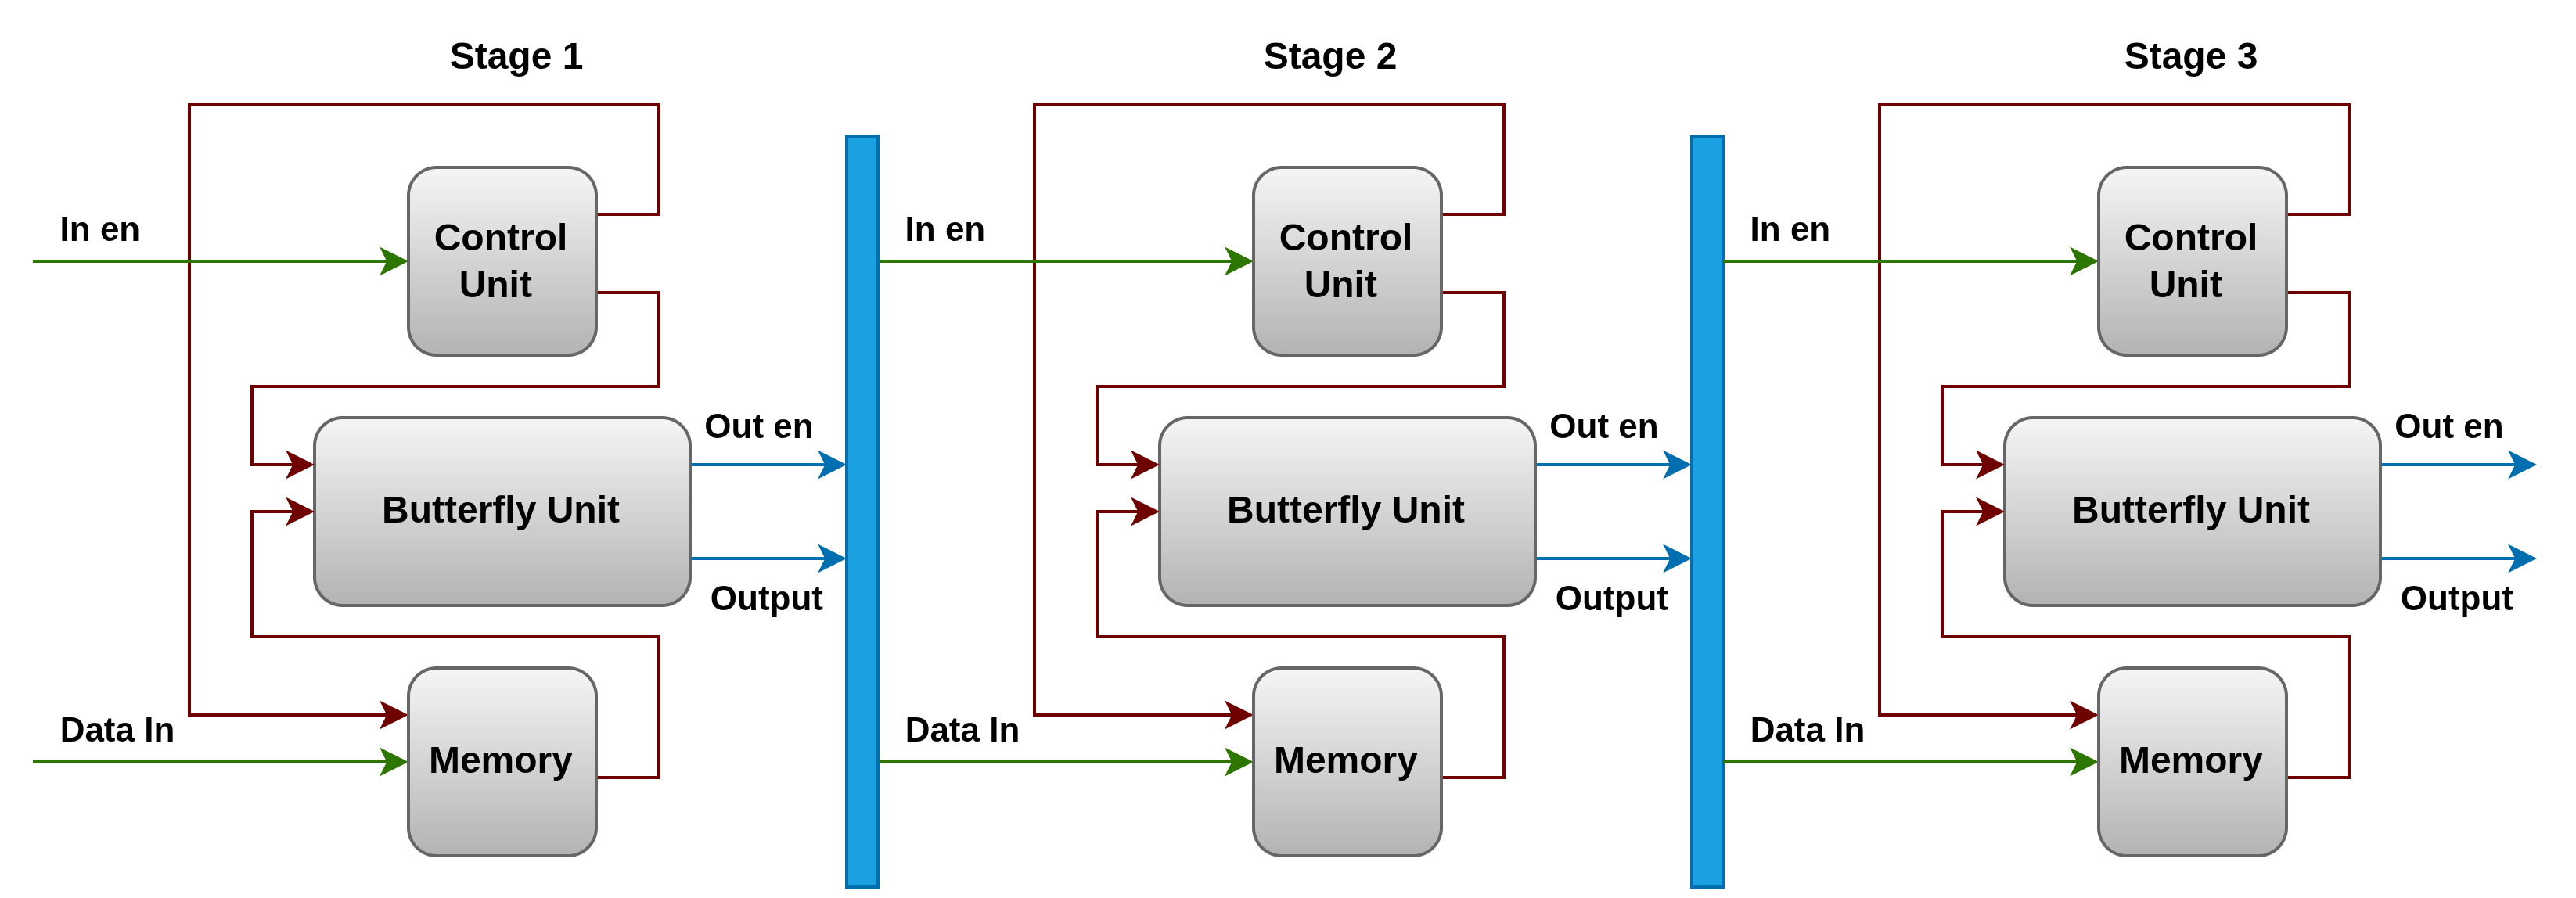
\includegraphics[width=1\linewidth]{Images/SDF_unit.png}
    \caption{Simplified diagram of the SDF units discussed in this chapter.}
    \label{fig:sdf_unit_intro}
\end{figure}

\section{Fixed-Point Arithmetic and Quantization Noise}
In hardware implementations of the FFT, floating-point arithmetic is typically avoided due to its high resource consumption and latency. Instead, signals and twiddle factors are represented using fixed-point formats, such as the Q format. For instance, a 32-bit data path might utilize a Q1.15 effective scaling, where a value of 1.0 corresponds to the integer 32767. The mathematical representation of this quantization scales a continuous signal $x(t)$ by a factor of $2^{W-1}-1$, where $W$ is the word length.  

Because fixed-point variables have finite precision, rounding or truncation occurs after mathematical operations, particularly after complex multiplications with twiddle factors. This introduces a small amount of error known as quantization noise. This error accumulates with every successive stage of the FFT.
The degradation is evaluated using the Signal-to-Quantization-Noise Ratio (SQNR), which compares the power of the original signal to the power of the quantization noise.

\begin{figure}[htbp]
    \centering
    \vspace{1em}
    
    % Power equation
    $\displaystyle P_{x^\nu} = 10\log_{10} \left( \frac{1}{N} \sum_{n=0}^{N-1} |x[n]|^2 \right)$
    
    \vspace{1.5em}
    
    % SQNR equation
    $\displaystyle \text{SQNR}|_{dB} = P_{x^\nu} + 6.02\nu + 4.77$
    
    \vspace{1em}
    \caption{Formulas for the signal power and Signal-to-Quantization-Noise Ratio (SQNR). $P_{x^\nu}$ represents the average power of the input signal. $\nu$ represents the number of bits (resolution).}
    \label{fig:sqnr_and_power}
\end{figure}

To determine the absolute maximum SQNR for a given bit depth, we assume a full-scale square input wave, which provides a normalized linear average power of 1 ($10\log_{10}(1) = 0$ dB). Consequently, for a 16-bit resolution, the maximum achievable SQNR is 101.09 dB. Table \ref{tab:max_sqnr} demonstrates the theoretical maximum SQNR limits across common hardware bit depths.

\begin{table}[htbp]
    \centering
    \caption{Maximum theoretical SQNR for various hardware bit depths (assuming full-scale square wave input).}
    \vspace{0.5em}
    \begin{tabular}{|c|c|}
        \hline
        \textbf{Resolution ($\nu$ bits)} & \textbf{Maximum SQNR (dB)} \\
        \hline
        8 & 52.93 \\
        12 & 77.01 \\
        16 & 101.09 \\
        \hline
    \end{tabular}
    \label{tab:max_sqnr}
\end{table}

\section{Custom Multipliers}
This thesis implements two distinct custom multiplier architectures: a generic carry-save array multiplier for general arithmetic operations and a specialized computation-sharing multiplier (CSHM) optimized for signal processing workloads.

\subsection{Carry-Save Array Multiplier}

A Carry-Save Array Multiplier (CSAM) accelerates arithmetic by eliminating the intermediate carry-propagation delays found in standard array multipliers. The operation consists of three main stages:

\begin{enumerate}
    \item \textbf{Partial Product Generation:} A matrix of partial products is created using logical AND gates between the multiplicand and multiplier bits.
    \item \textbf{Carry-Save Reduction:} Instead of rippling carries horizontally across rows, Carry-Save Adders (CSAs) are used. Each CSA passes independent sum and carry bits diagonally down to the next row, keeping the intermediate results as two unmerged vectors.
    \item \textbf{Final Addition:} A traditional carry-propagate adder is used only at the very last stage to merge the final sum and carry vectors into the resolved product.
\end{enumerate}

By breaking the horizontal carry chain during intermediate steps, the CSAM reduces the critical path delay while maintaining a highly regular hardware structure suitable for FPGAs.

\begin{figure}[H]
    \centering
    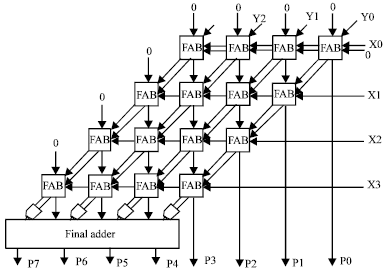
\includegraphics[width=0.6\linewidth]{Images/Carry-Save-Multiplier.png}
    \caption{Top diagram of the Carry-Save Array Multiplier discussed in this chapter}
    \label{fig:Carry-Save Mult}
\end{figure}

\subsection{Computation-Sharing Hardware Multiplier (CSHM)}

The Computation-Sharing Hardware Multiplier (CSHM) minimizes hardware logic by identifying and reusing redundant partial products. It is highly efficient for signal processing tasks where a single input data stream is multiplied by various coefficients.

\begin{itemize}
    \item \textbf{Alphabets and Sets:} CSHM simplifies multiplication by decomposing coefficients into a small set of recurring factor patterns, known as an \textit{alphabet}. A common basis set consists of small odd integers, such as $\{1, 3, 5, 7\}$. The architecture precomputes the multiplicand against this limited set of values.
    \item \textbf{Addition and Assembly:} Generating the initial alphabet set requires minimal hardware (e.g., $3x$ is computed as $2x + x$, requiring just one shift and one adder). The final multiplication product is then reconstructed by selecting, shifting, and adding these precomputed set values together. This computation-sharing approach drastically reduces the total number of resources and latency required compared to a classical multiplier.
\end{itemize}

\begin{figure}[H]
    \centering
    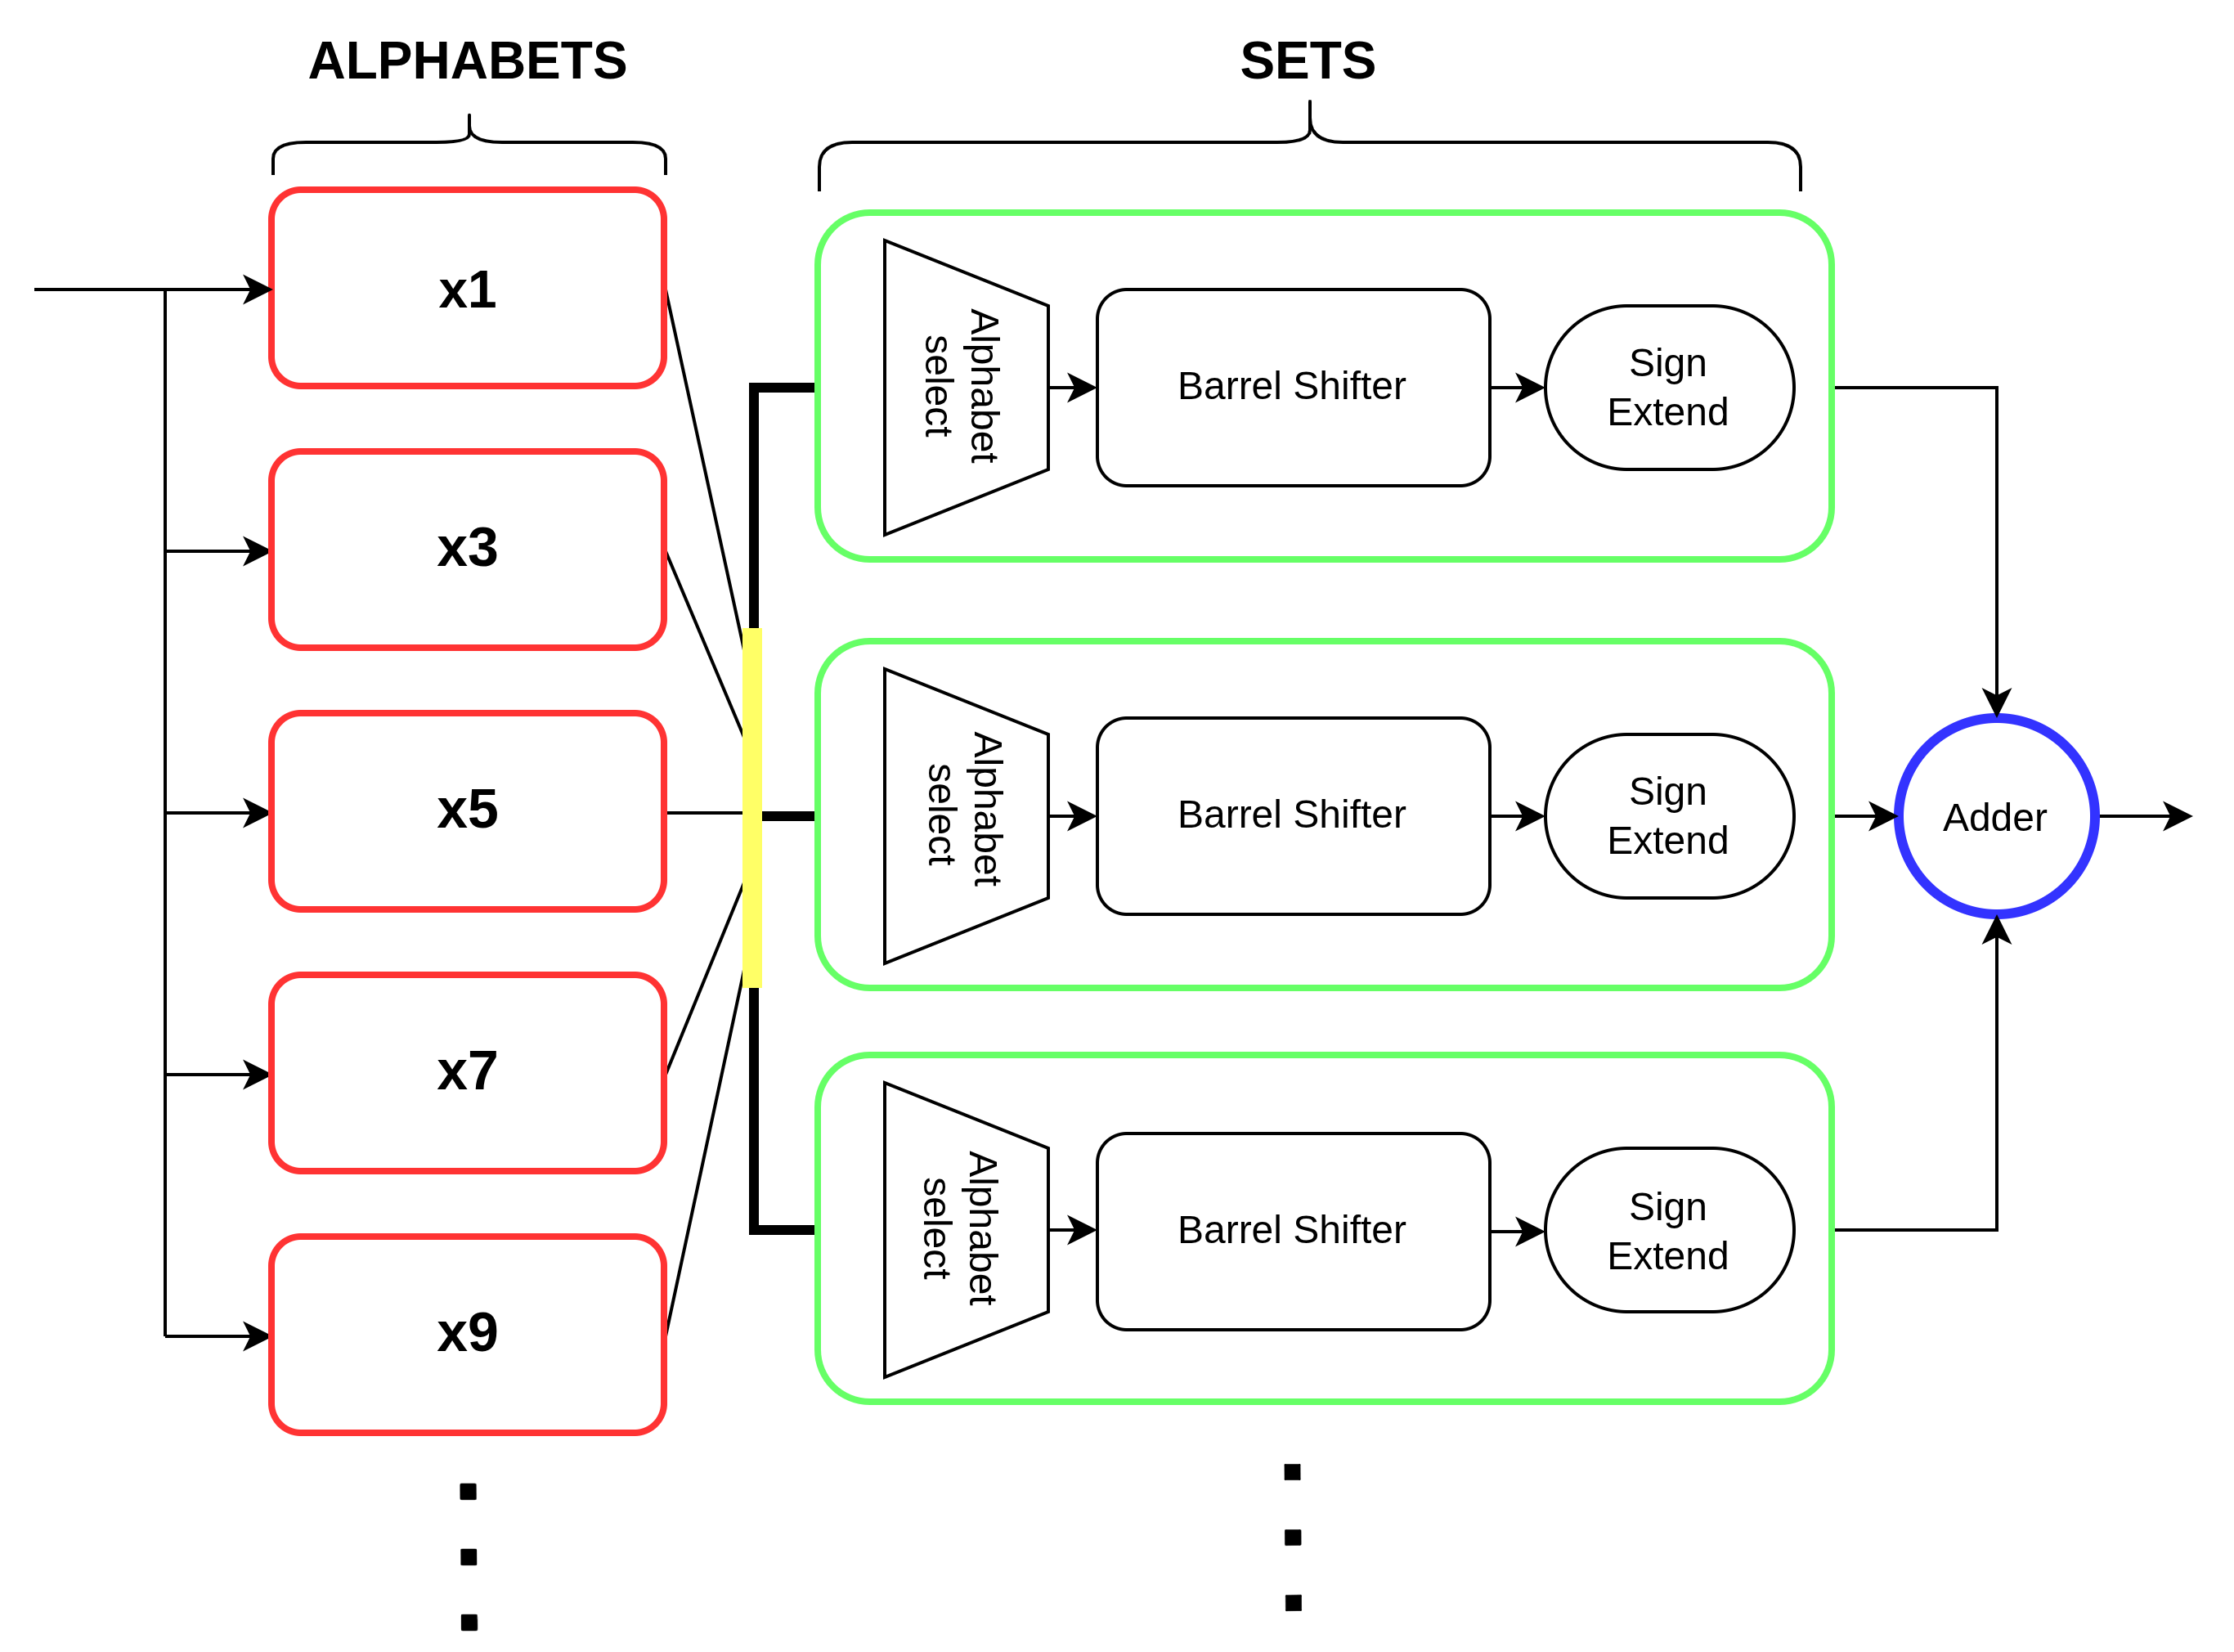
\includegraphics[width=0.8\linewidth]{Images/CSHM_gen.drawio.png}
    \caption{Top diagram of the CSHM Multiplier discussed in this chapter}
    \label{fig:Cshm general Unit}
\end{figure}

\begin{itemize}
    \item \textbf{Examples:}
    
        \textbf{Using a 2-Bit Set ($\{1, 3\}$):} Consider multiplying an input $x$ by the coefficient $27$ (binary $011011_2$). The coefficient is partitioned into 2-bit slices: $01_2$ (1), $10_2$ (2), and $11_2$ (3). The multiplication is reconstructed as $(1x \cdot 2^4) + (1x \cdot 2^3) + (3x \cdot 2^0)$. The hardware routes and shifts the precomputed $1x$ and $3x$ values, avoiding full multipliers.\\
        \textbf{Using a 3-Bit Set ($\{1, 3, 5, 7\}$):} Consider multiplying an input $x$ by the coefficient $45$ (binary $101101_2$). The coefficient is partitioned into 3-bit slices: $101_2$ (5) and $101_2$ (5). The multiplication is reconstructed as $(5x \cdot 2^3) + (5x \cdot 2^0)$. The hardware only needs to compute the partial product $5x$ once, sharing that computation for both halves of the coefficient.
\end{itemize}

\section{FPGA Hardware Resources}

Modern Field-Programmable Gate Arrays (FPGAs) provide dedicated architectural primitives to accelerate digital signal processing algorithms and manage data streams efficiently. The hardware implementation of the proposed FFT and custom multipliers relies heavily on three core resources:

\begin{itemize}
    \item \textbf{Digital Signal Processing (DSP) Blocks:} These are dedicated, hard-silicon arithmetic units embedded within the FPGA fabric (such as DSP48 slices in AMD/Xilinx architectures~\cite{ug479}). They are optimized to perform high-speed, wide-bit operations like multiply-accumulate (MAC) and pre-addition.
    
    \item \textbf{Block RAM (BRAM):} BRAMs are dedicated memory blocks~\cite{ug473} arranged in columns throughout the FPGA. They provide high-capacity, synchronous data storage and can be configured as single-port or dual-port memories.
    
    \item \textbf{Look-Up Table RAM (LUTRAM) / Distributed RAM:} LUTRAM is generated by the logic Look-Up Tables (LUTs) in the general logic fabric~\cite{ug473} to act as small memory elements. While it provides less capacity than a BRAM, LUTRAM is placed directly next to logic cells, making it efficient for implementing small memory structures.
\end{itemize}